%----------------------------------------------------------------------
% Results

\begingroup
\allowdisplaybreaks

\section{Results}

\subsection{Traditional Calibration Sequence}

A traditional calibration sequence was simulated for a UUT with an assumed sample rate of $100 \,\unit{\hertz}$. Each test specified in table \ref{tab: traditional_calibration_tests} for a duration of $10 \,\unit{\second}$. All of the accelerometer test data were appended together to build the model operator $G_a$, and as well as all of the gyroscope test data to build $G_g$. Before proceeding with solving for the weighted least squares solution, a quick check was performed to ensure the both $G_a$ and $G_g$ were full rank. 

\begin{align}
	\textrm{rank}\left(G_a\right) &= 6,\,\,\, G_a \in \R^{60006 \times 12} \notag\\
	\\
	\textrm{rank}\left(G_g\right) &= 6,\,\,\, G_g \in \R^{60006 \times 12} \notag
\end{align}

The fact that both $G_a$ and $G_g$ are not full rank was not initially expected. However, given that the number of observations $m = 60006$ actually has many repeated rows as the UUT itself undergoes no changes in specific force and angular rate, this should not have been as much of a surprise. Instead of proceeding with solving for a solution, another calibration sequence was designed.







%******************************************************
% Single-Axis Motion
%******************************************************

\subsection{Single-Axis Motion Calibration Sequence}

In response to the lack of full rank in the previous experiment design, a new calibration sequence was designed to put axis of the UUT in motion in hopes of establishing model operators of full rank. Figures \ref{fig: single-axis angular velocity profile} and \ref{fig: single-axis euler angle profile} show the designed motion profile.

\begin{figure}[h] 
	\centering
	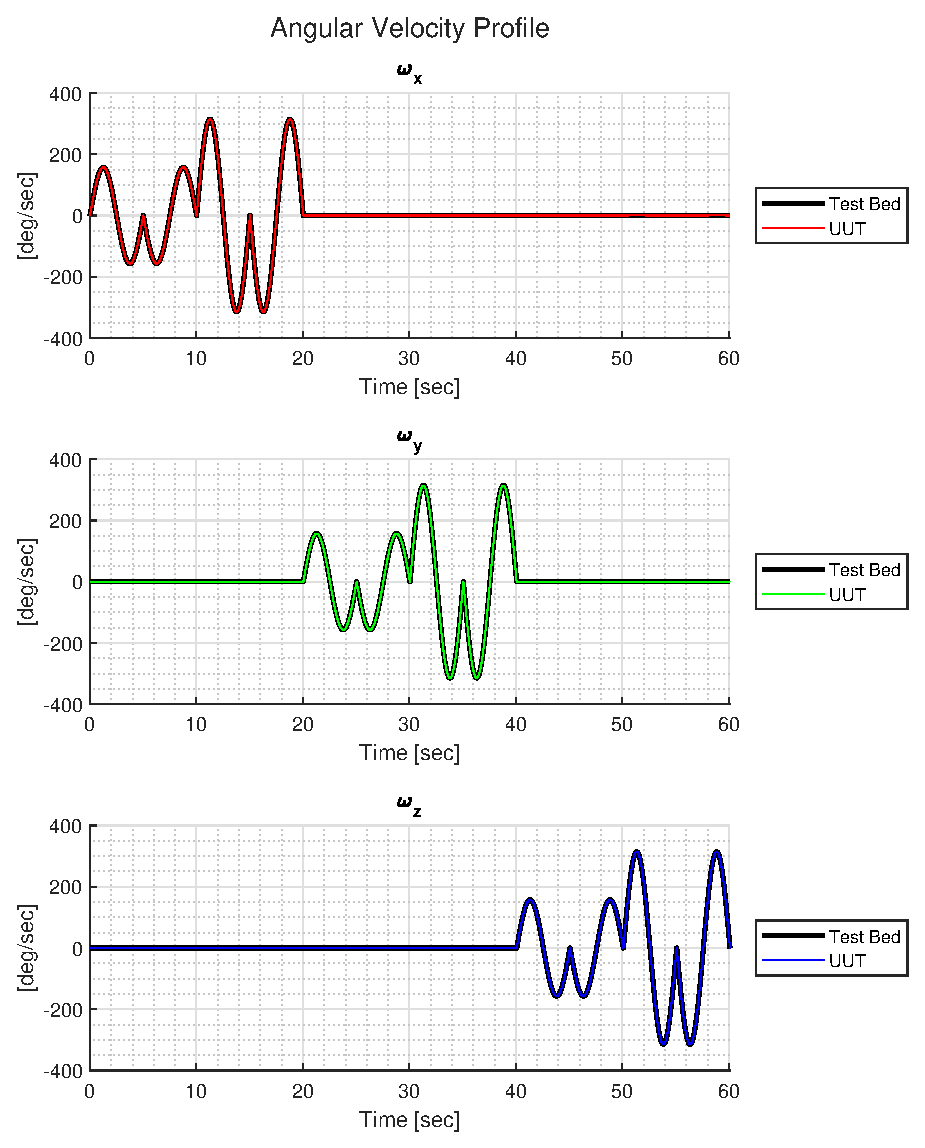
\includegraphics[width=0.65\textwidth]{./images/SAM_angular_velocity_profile.eps}
	\caption{Single-Axis Angular Velocity Profile}
	\label{fig: single-axis angular velocity profile}
\end{figure}
\FloatBarrier

\begin{figure}[h] 
	\centering
	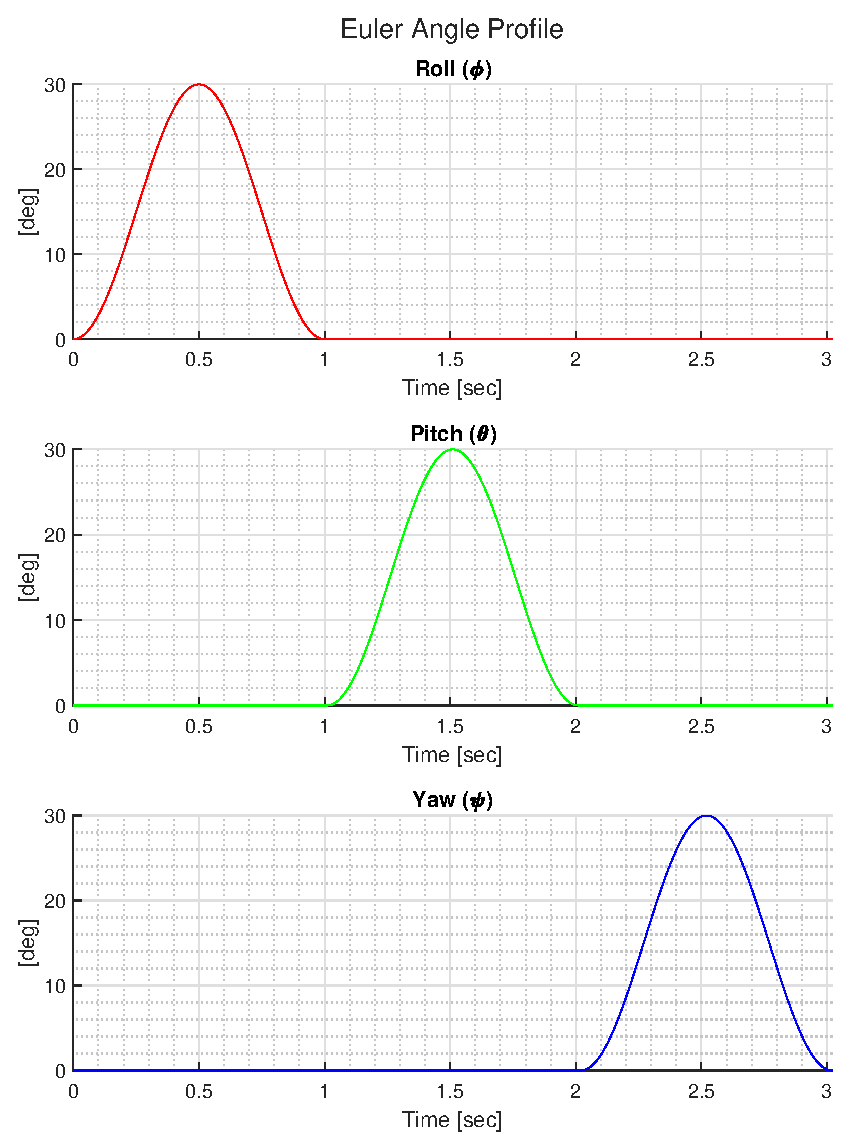
\includegraphics[width=0.65\textwidth]{./images/SAM_euler_angle_profile.eps}
	\caption{Single-Axis Euler Angle Profile}
	\label{fig: single-axis euler angle profile}
\end{figure}
\FloatBarrier

Due to the rotations of the test bed, the specific force is also altered as shown in figure \ref{fig: single-axis specific force profile}.

\begin{figure}[h] 
	\centering
	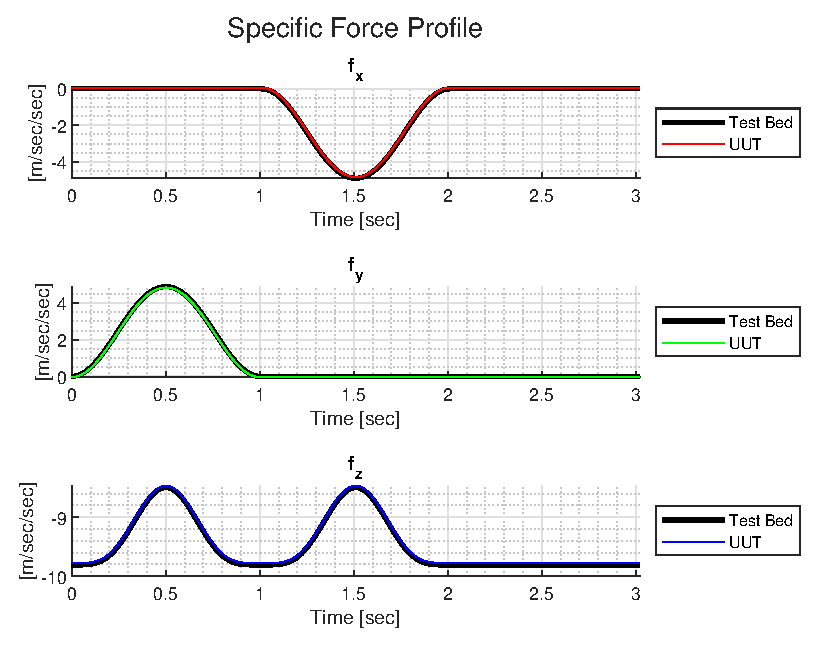
\includegraphics[width=0.65\textwidth]{./images/SAM_specific_force_profile.eps}
	\caption{Single-Axis Specific Force Profile}
	\label{fig: single-axis specific force profile}
\end{figure}
\FloatBarrier

\subsubsection{Model Operator Rank}

Even with new motion profiles, both model operators $G_a$ and $G_g$ are not full rank. 

\begin{align}
	\textrm{rank}\left(G_a\right) &= 12,\,\,\, G_a \in \R^{909 \times 12} \notag\\
	\\
	\textrm{rank}\left(G_g\right) &= 12,\,\,\, G_g \in \R^{909 \times 12} \notag
\end{align}

In response, a model solution was still obtained using the generalized inverse. This rank-deficiency is of the type "$p = n$ and $p < m$, in which the data null space is non-trivial but the model null space is trivial. This implies that the solution will be unique, but cannot fit the general data exactly. For both $G_a$ and $G_g$, a singular value decomposition (SVD) was performed and each decomposed matrix was truncated to the rank of the matrix. The generalized inverse model was formed accordingly below.

\begin{align}
	\bv{m}_{\dagger}^{a} &= V_{a,p} S_{a,p}^{-1} U_{a,p}^T \bv{d}_a \notag\\
	\\
	\bv{m}_{\dagger}^{g} &= V_{g,p} S_{g,p}^{-1} U_{g,p}^T \bv{d}_g \notag
\end{align}

Each model resolution matrix $R_m = V_p V_p^T$ shows that each model parameter has perfect resolution. The singular values for each model operator are shown in figures \ref{fig: single-axis accelerometer singular values} and \ref{fig: single-axis gyroscope singular values}. 

\begin{figure}[h] 
	\centering
	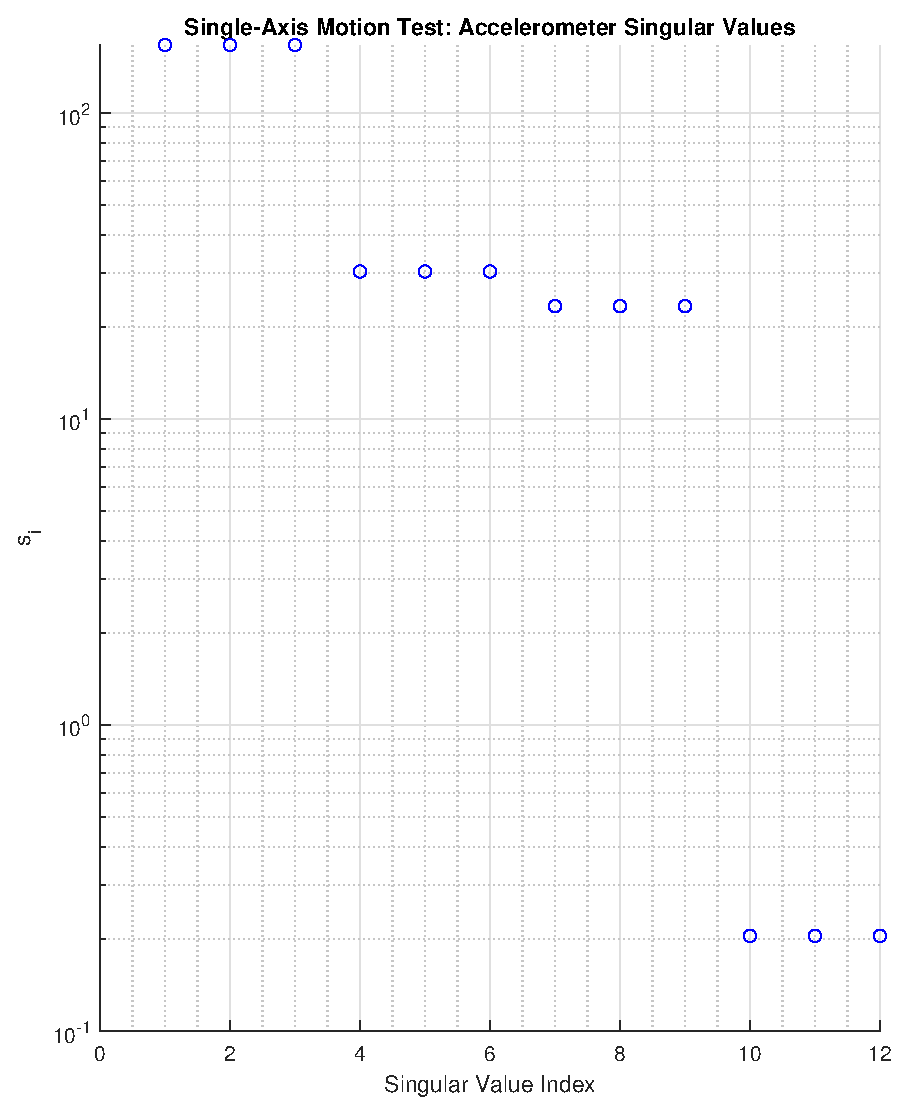
\includegraphics[width=0.65\textwidth]{./images/SAM_accel_singular_values.eps}
	\caption{Accelerometer Singular Values}
	\label{fig: single-axis accelerometer singular values}
\end{figure}
\FloatBarrier

\begin{figure}[h] 
	\centering
	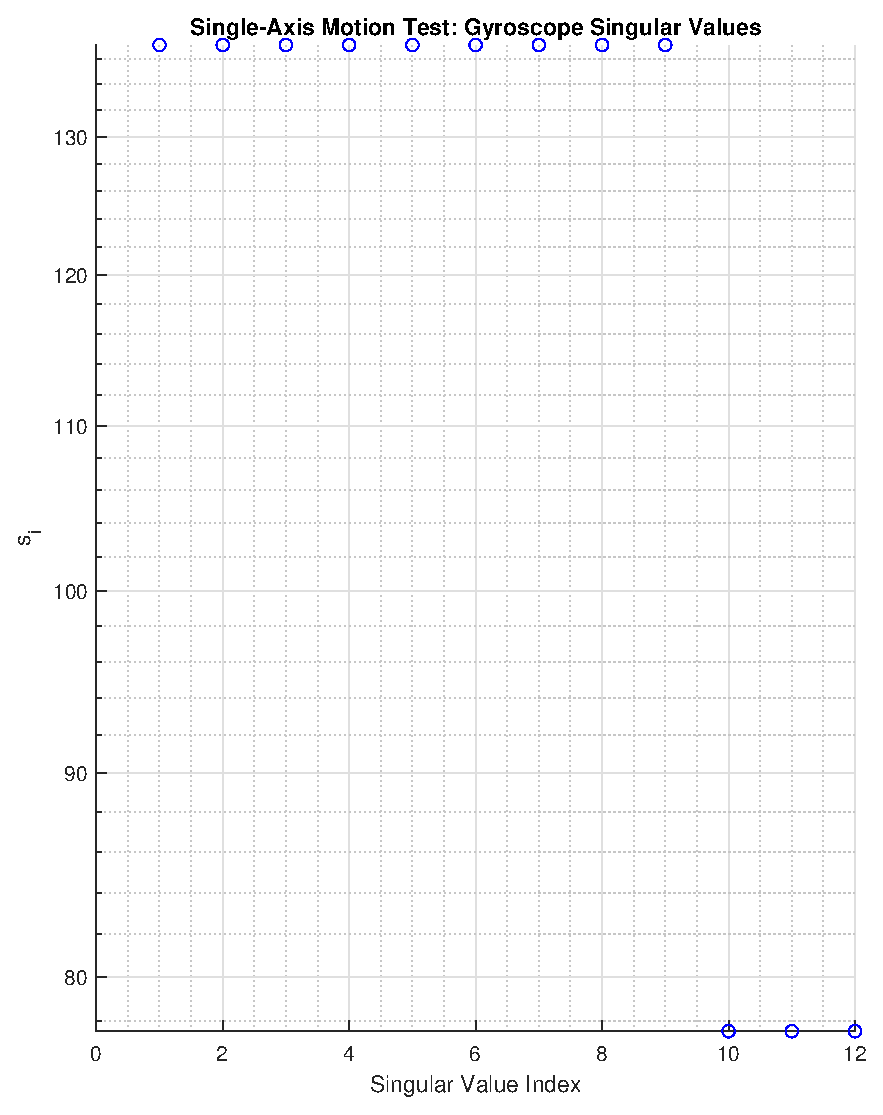
\includegraphics[width=0.65\textwidth]{./images/SAM_gyro_singular_values.eps}
	\caption{Gyroscope Singular Values}
	\label{fig: single-axis gyroscope singular values}
\end{figure}
\FloatBarrier


\subsubsection{Estimated Model Parameters}

The estimated model parameters and their associated errors are provided in figures \ref{fig: single-axis accelerometer parameters}, \ref{fig: single-axis accelerometer parameter error}, \ref{fig: single-axis gyroscope parameters}, and \ref{fig: single-axis gyroscope parameter error}. 

\begin{figure}[h] 
	\centering
	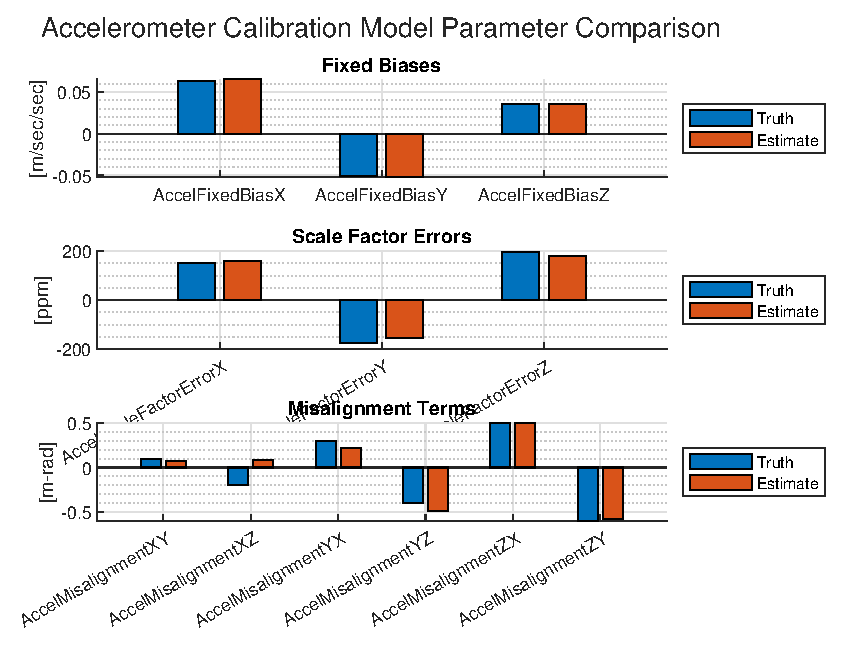
\includegraphics[width=0.65\textwidth]{./images/SAM_accel_model_parameters.eps}
	\caption{Estimated Accelerometer Model Parameters}
	\label{fig: single-axis accelerometer parameters}
\end{figure}
\FloatBarrier

\begin{figure}[h] 
	\centering
	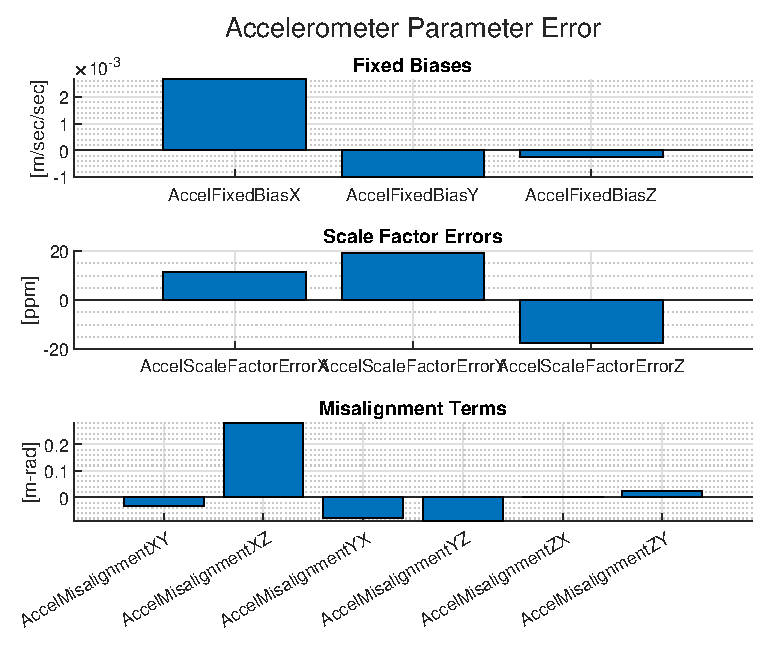
\includegraphics[width=0.65\textwidth]{./images/SAM_accel_model_error.eps}
	\caption{Accelerometer Model Parameter Error}
	\label{fig: single-axis accelerometer parameter error}
\end{figure}
\FloatBarrier

\begin{figure}[h] 
	\centering
	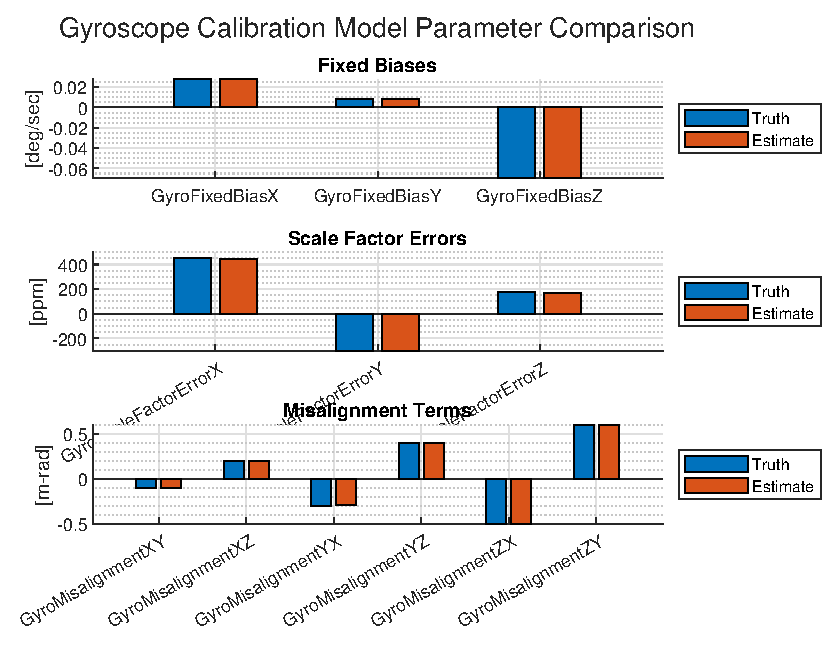
\includegraphics[width=0.65\textwidth]{./images/SAM_gyro_model_parameters.eps}
	\caption{Estimated Gyroscope Model Parameters}
	\label{fig: single-axis gyroscope parameters}
\end{figure}
\FloatBarrier

\begin{figure}[h] 
	\centering
	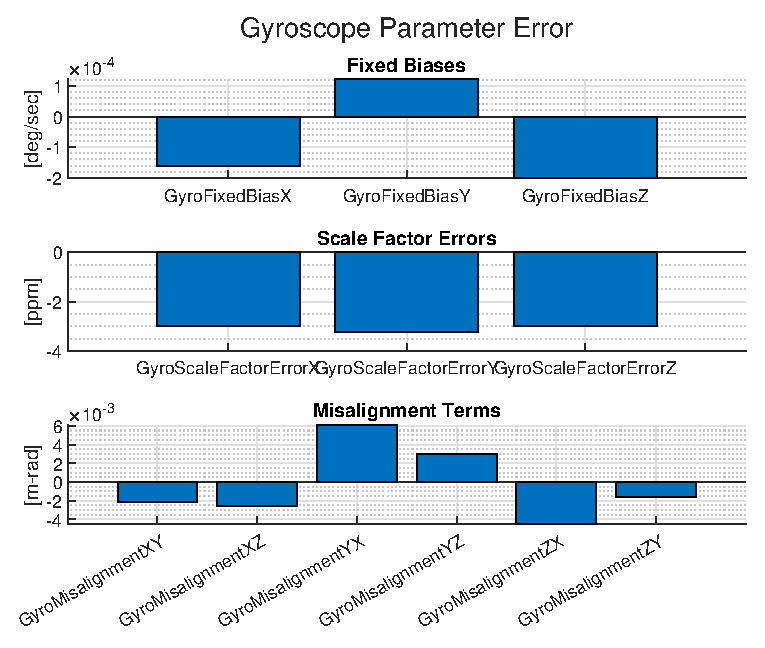
\includegraphics[width=0.65\textwidth]{./images/SAM_gyro_model_error.eps}
	\caption{Gyroscope Model Parameter Error}
	\label{fig: single-axis gyroscope parameter error}
\end{figure}
\FloatBarrier


\subsubsection{Model Covariance and 95\% Confidence Bounds}

In preparation for formulating a weighted least squares solution, the weighted matrices were used to compute the model covariance and resulting 95\% confidence bounds. 

\begin{figure}[h] 
	\centering
	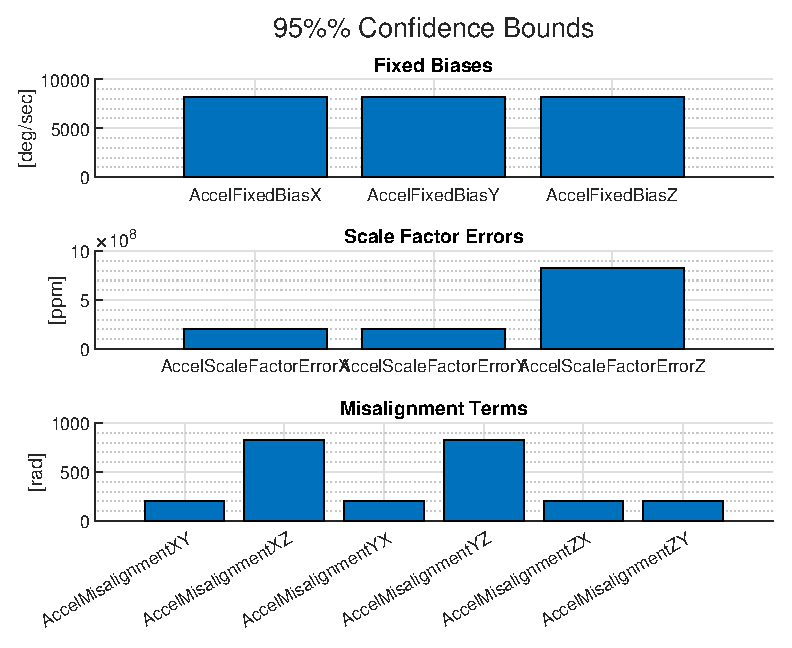
\includegraphics[width=0.65\textwidth]{./images/SAM_accel_model_95_confidence_bounds.eps}
	\caption{Accelerometer 95\% Confidence Bounds}
	\label{fig: single-axis accel 95 confidence bounds}
\end{figure}
\FloatBarrier

\begin{figure}[h] 
	\centering
	\includegraphics[width=0.65\textwidth]{./images/SAM_gyro_model_95_confidence_bounds.eps}
	\caption{Gyroscope 95\% Confidence Bounds}
	\label{fig: single-axis gyro 95 confidence bounds}
\end{figure}
\FloatBarrier

In each case, the confidence bounds are wildly higher than the error actually achieved through the generalized model inverse solution!
















%******************************************************
% Multi-Axis Motion
%******************************************************

\subsection{Multi-Axis Motion Calibration Sequence}

In response to still lacking full rank with the single-axis motion calibration sequences, yet another calibration sequence was designed to put axis of the UUT in motion at the same time in hopes of establishing model operators of full rank. Figures \ref{fig: multi-axis angular velocity profile} and \ref{fig: multi-axis euler angle profile} show the designed motion profile.

\begin{figure}[h] 
	\centering
	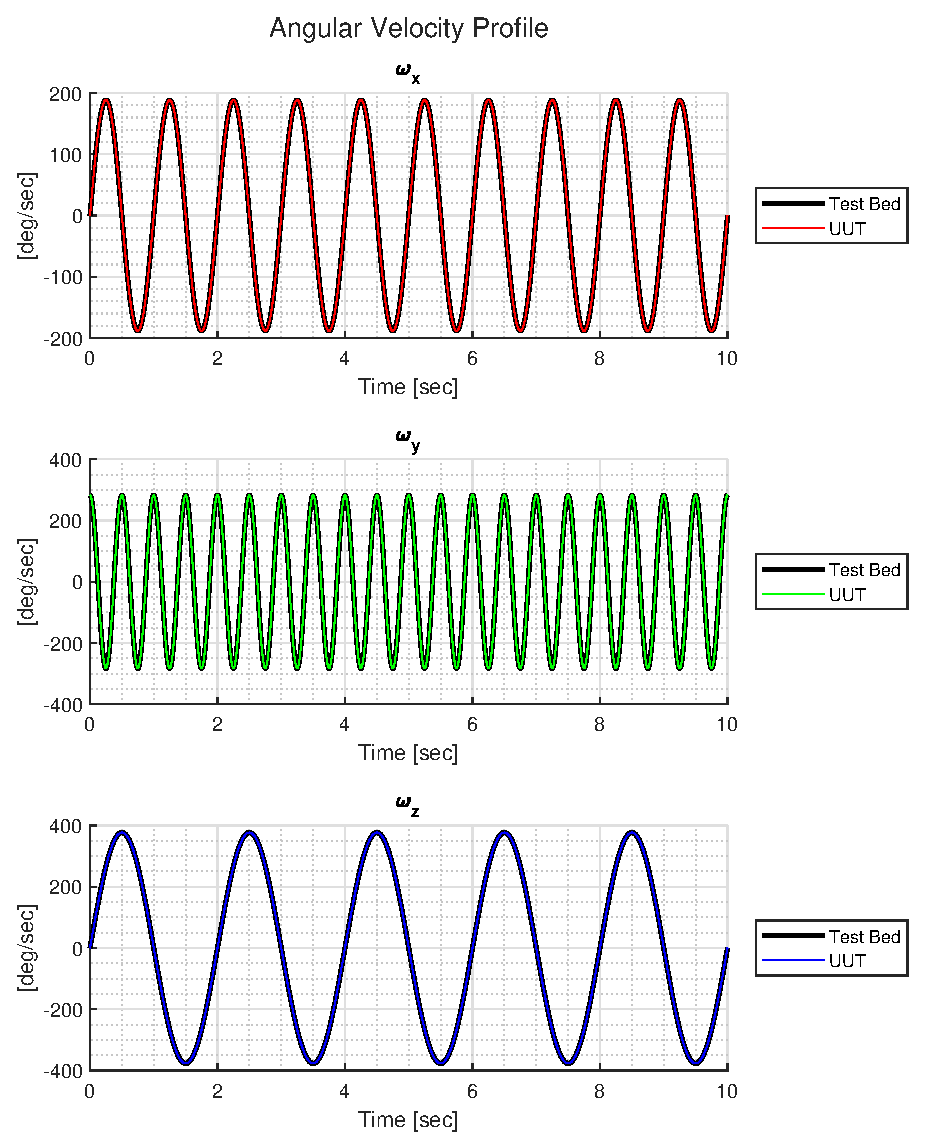
\includegraphics[width=0.65\textwidth]{./images/MAM_angular_velocity_profile.eps}
	\caption{Multi-Axis Angular Velocity Profile}
	\label{fig: multi-axis angular velocity profile}
\end{figure}
\FloatBarrier

\begin{figure}[h] 
	\centering
	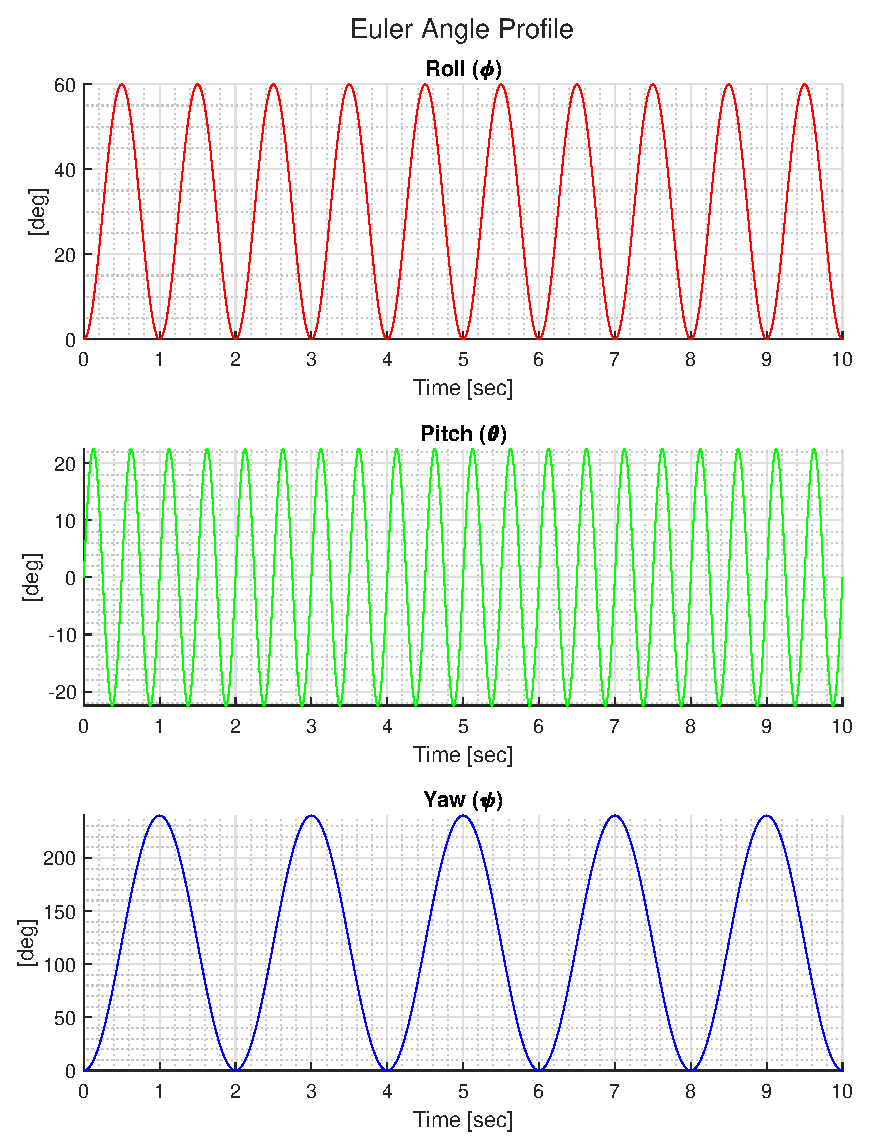
\includegraphics[width=0.65\textwidth]{./images/MAM_euler_angle_profile.eps}
	\caption{Multi-Axis Euler Angle Profile}
	\label{fig: multi-axis euler angle profile}
\end{figure}
\FloatBarrier

Due to the rotations of the test bed, the specific force is also altered as shown in figure \ref{fig: multi-axis specific force profile}.

\begin{figure}[h] 
	\centering
	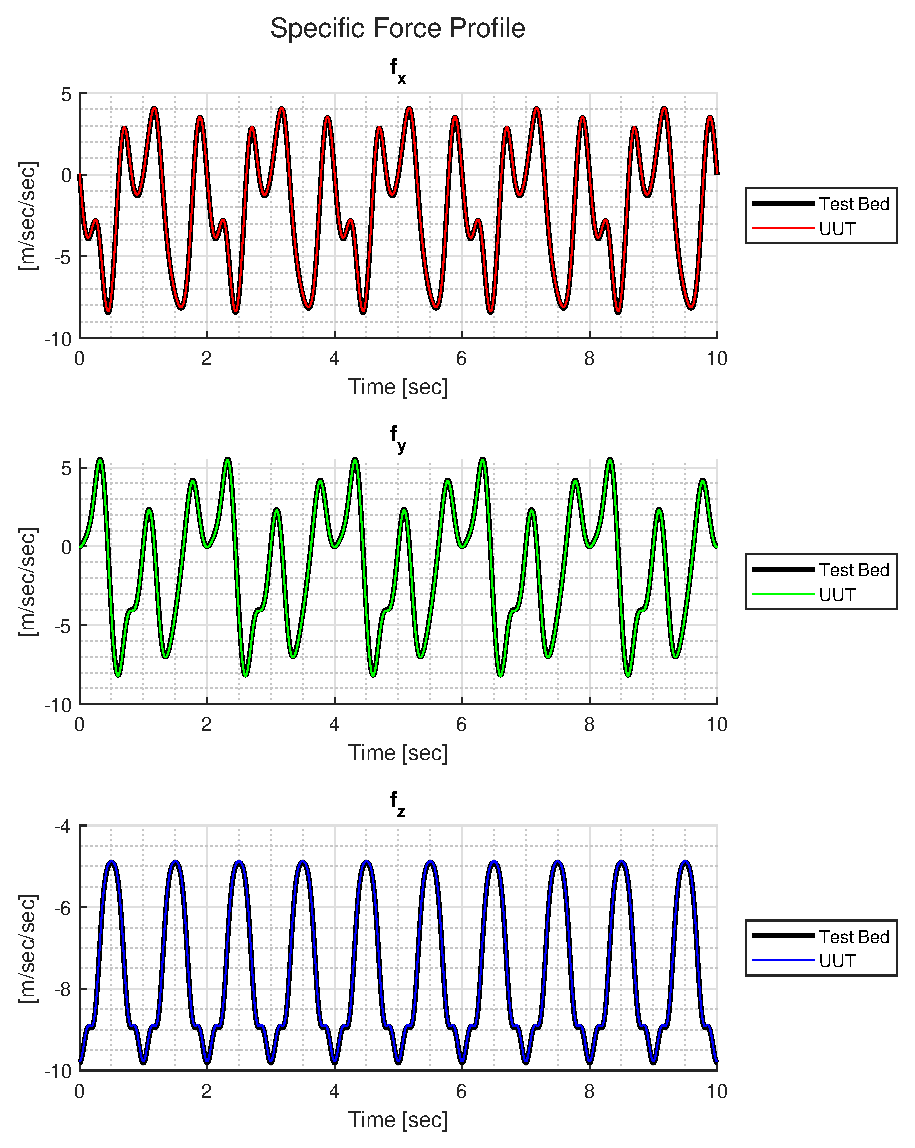
\includegraphics[width=0.65\textwidth]{./images/MAM_specific_force_profile.eps}
	\caption{Multi-Axis Specific Force Profile}
	\label{fig: multi-axis specific force profile}
\end{figure}
\FloatBarrier

\subsubsection{Model Operator Rank}

Even with new motion profiles, both model operators $G_a$ and $G_g$ are not full rank. 

\begin{align}
	\textrm{rank}\left(G_a\right) &= 12,\,\,\, G_a \in \R^{909 \times 12} \notag\\
	\\
	\textrm{rank}\left(G_g\right) &= 12,\,\,\, G_g \in \R^{909 \times 12} \notag
\end{align}

In response, a model solution was still obtained using the generalized inverse. This rank-deficiency is of the type "$p = n$ and $p < m$, in which the data null space is non-trivial but the model null space is trivial. This implies that the solution will be unique, but cannot fit the general data exactly. For both $G_a$ and $G_g$, a singular value decomposition (SVD) was performed and each decomposed matrix was truncated to the rank of the matrix. The generalized inverse model was formed accordingly below.

\begin{align}
	\bv{m}_{\dagger}^{a} &= V_{a,p} S_{a,p}^{-1} U_{a,p}^T \bv{d}_a \notag\\
	\\
	\bv{m}_{\dagger}^{g} &= V_{g,p} S_{g,p}^{-1} U_{g,p}^T \bv{d}_g \notag
\end{align}

Each model resolution matrix $R_m = V_p V_p^T$ shows that each model parameter has perfect resolution. The singular values for each model operator are shown in figures \ref{fig: multi-axis accelerometer singular values} and \ref{fig: multi-axis gyroscope singular values}. 

\begin{figure}[h] 
	\centering
	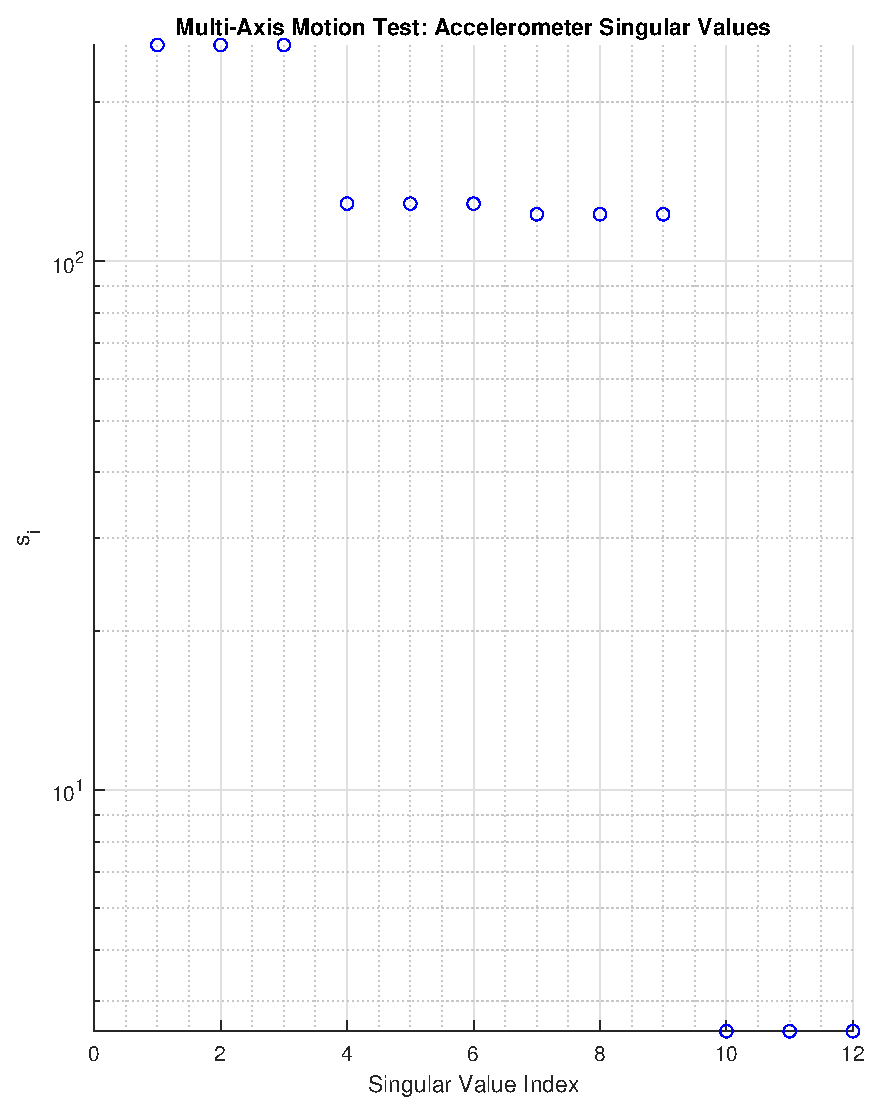
\includegraphics[width=0.65\textwidth]{./images/MAM_accel_singular_values.eps}
	\caption{Accelerometer Singular Values}
	\label{fig: multi-axis accelerometer singular values}
\end{figure}
\FloatBarrier

\begin{figure}[h] 
	\centering
	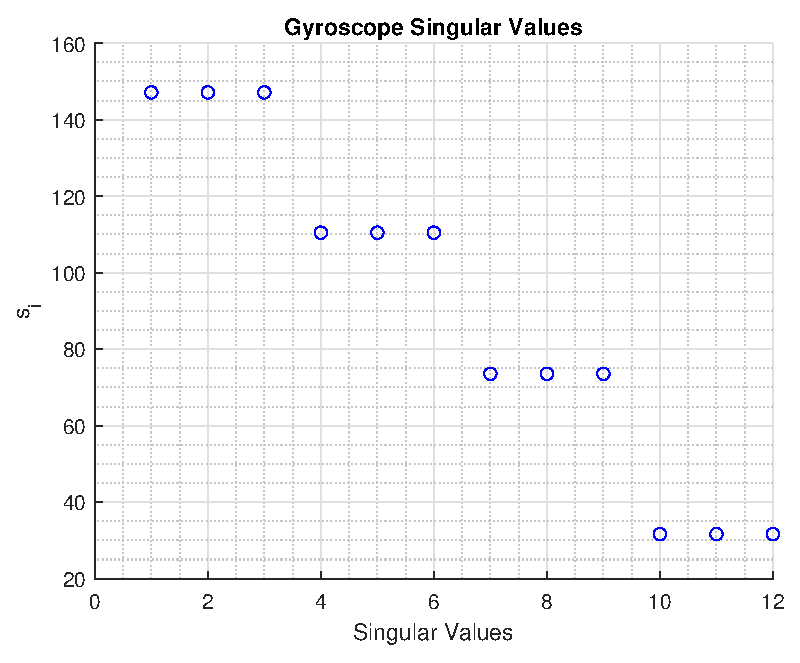
\includegraphics[width=0.65\textwidth]{./images/MAM_gyro_singular_values.eps}
	\caption{Gyroscope Singular Values}
	\label{fig: multi-axis gyroscope singular values}
\end{figure}
\FloatBarrier


\subsubsection{Estimated Model Parameters}

The estimated model parameters and their associated errors are provided in figures \ref{fig: multi-axis accelerometer parameters}, \ref{fig: multi-axis accelerometer parameter error}, \ref{fig: multi-axis gyroscope parameters}, and \ref{fig: multi-axis gyroscope parameter error}. 

\begin{figure}[h] 
	\centering
	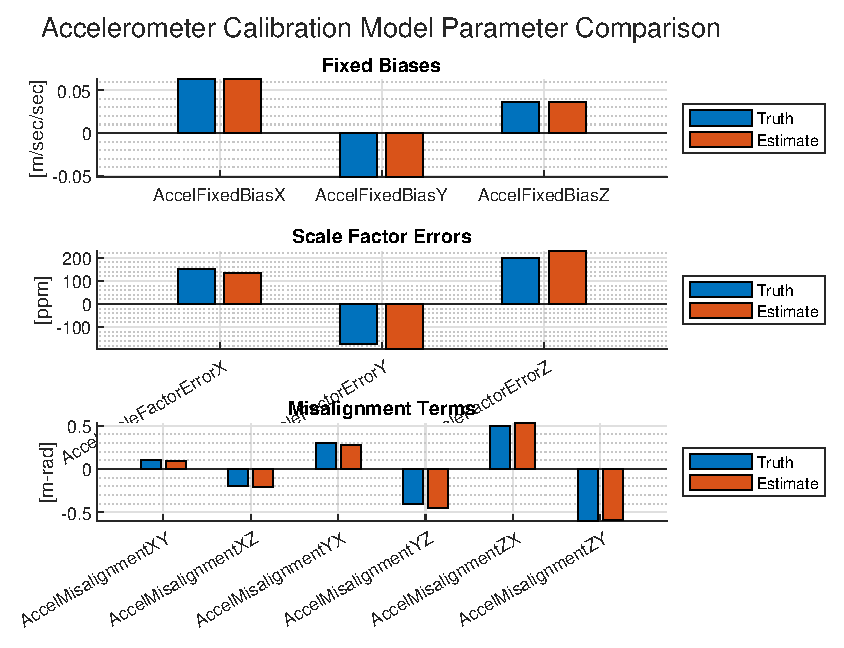
\includegraphics[width=0.65\textwidth]{./images/MAM_accel_model_parameters.eps}
	\caption{Estimated Accelerometer Model Parameters}
	\label{fig: multi-axis accelerometer parameters}
\end{figure}
\FloatBarrier

\begin{figure}[h] 
	\centering
	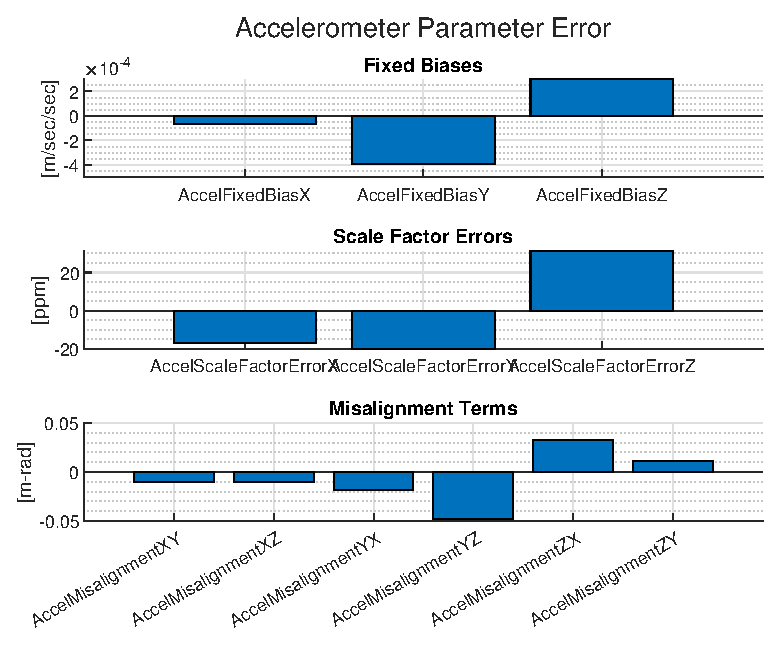
\includegraphics[width=0.65\textwidth]{./images/MAM_accel_model_error.eps}
	\caption{Accelerometer Model Parameter Error}
	\label{fig: multi-axis accelerometer parameter error}
\end{figure}
\FloatBarrier

\begin{figure}[h] 
	\centering
	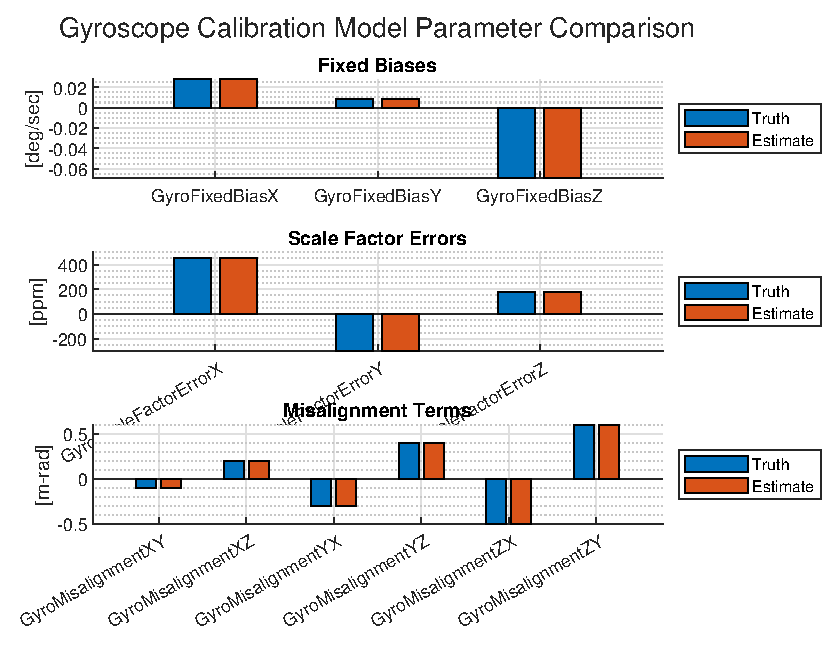
\includegraphics[width=0.65\textwidth]{./images/MAM_gyro_model_parameters.eps}
	\caption{Estimated Gyroscope Model Parameters}
	\label{fig: multi-axis gyroscope parameters}
\end{figure}
\FloatBarrier

\begin{figure}[h] 
	\centering
	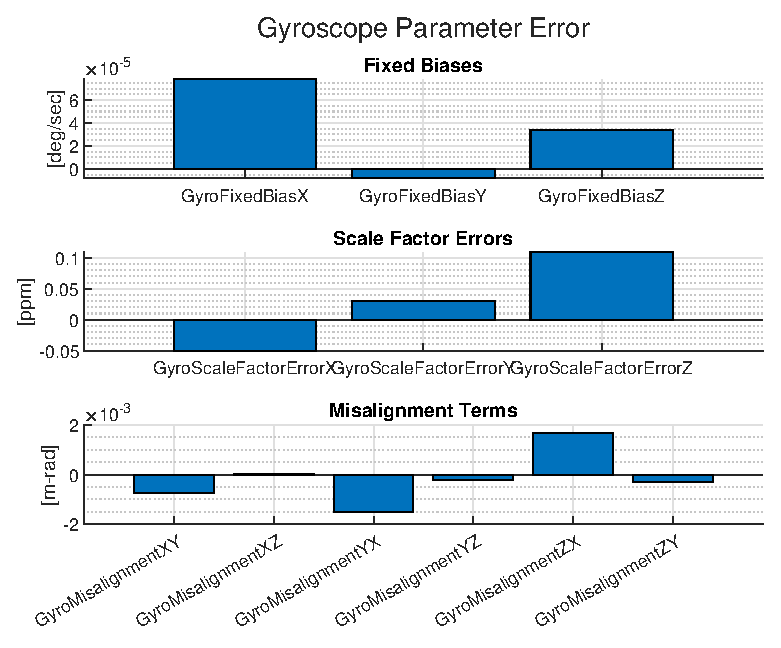
\includegraphics[width=0.65\textwidth]{./images/MAM_gyro_model_error.eps}
	\caption{Gyroscope Model Parameter Error}
	\label{fig: multi-axis gyroscope parameter error}
\end{figure}
\FloatBarrier


\subsubsection{Model Covariance and 95\% Confidence Bounds}

In preparation for formulating a weighted least squares solution, the weighted matrices were used to compute the model covariance and resulting 95\% confidence bounds. 

\begin{figure}[h] 
	\centering
	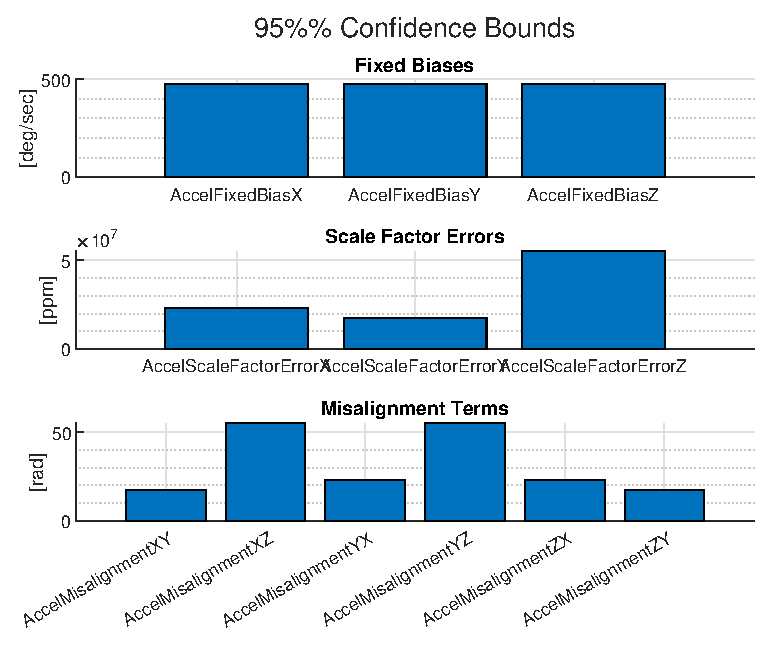
\includegraphics[width=0.65\textwidth]{./images/MAM_accel_model_95_confidence_bounds.eps}
	\caption{Accelerometer 95\% Confidence Bounds}
	\label{fig: multi-axis accel 95 confidence bounds}
\end{figure}
\FloatBarrier

\begin{figure}[h] 
	\centering
	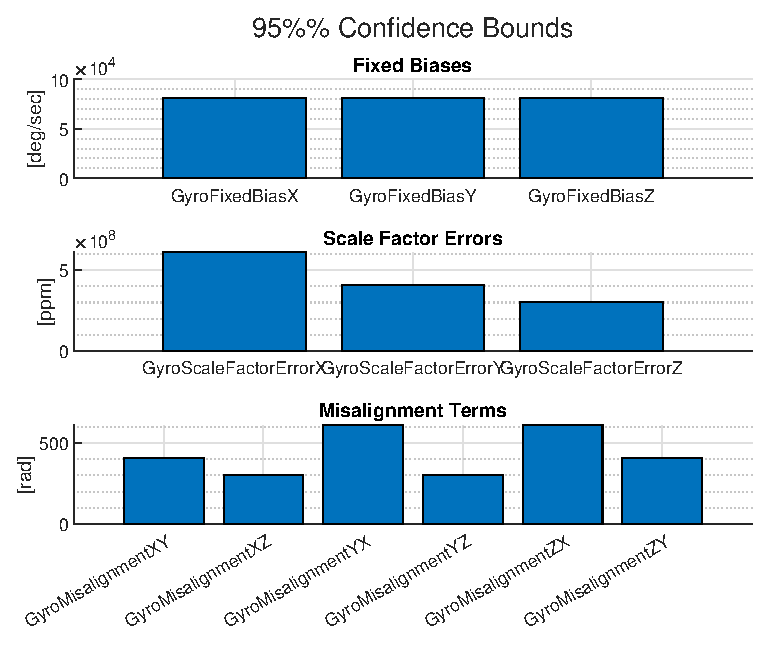
\includegraphics[width=0.65\textwidth]{./images/MAM_gyro_model_95_confidence_bounds.eps}
	\caption{Gyroscope 95\% Confidence Bounds}
	\label{fig: multi-axis gyro 95 confidence bounds}
\end{figure}
\FloatBarrier

In each case, the confidence bounds are wildly higher than the error actually achieved through the generalized model inverse solution!


